%!TEX root = main.tex
\graphicspath{{images/chap2/}}
% Related Literature and Studies
% * Organized to cover specific problem
% * how it helps the current study/how it relates
\chapter{Related Work} % (fold)
\label{cha:related_work}

\section{Image Recognition and Animal Biometric} % (fold)
\label{sec:image_recognition}

Animal pattern recognition is a specific case of object recognition.
The problem of finding matching image pairs from the database given an input
image can be reduced to following \emph{decision problem}:
\begin{quote}
\centering
Given two images $A$ and $B$, is the animal in image $A$ the same
individual as the animal in image $B$?
\end{quote}

The problem is somewhat similar to the face verification problem, which involves
accepting or rejecting an identity claim based on the image of a human face.
There are two major differences between animal identification and face
verification. First, the animal patterns have finer-grained details and some can
be very subtle such that they fuse into the background. Second, the pattern of
each individual does not share same overall structure as a human face does. This
is similar to identifying an identical twin by their blemishes, except in this
case, we have a very high-order of multiple births.

Typical feature-based image recognition methods fall into three main categories:
(1) generic methods, which involves edges, lines, and curves, (2)
feature-template-based methods, in which the locations of the key features are
used, (3) structural matching methods, which relies on geometrical
constraints~\cite{facesurvey03}.  We will only be focusing on the generic
methods of image recognition since the most discriminative features for animals
tend to be their patterns rather than their fiducial key features, i.e. eyes,
noses, or mouth.

A number of different generic feature extraction and classification strategies
have been used to recognize objects or faces from images, e.g. principal
components with nearest-neighbor~\cite{object91,object95,shape00}, support
vector machines~\cite{object97}, convolutional networks~\cite{object98} and
Scale Invariant Feature Transform (SIFT)~\cite{lowe04}. Computer-based animal
biometric methods extends these algorithms by emphasizing on discriminative
animal patterns. Standard generic approaches includes multi-scale differential
features~\cite{gamble08,ravela02,sloop13}, randomized
multiscale-PCA~\cite{ravela04}, SIFT~\cite{town13,sloop13}, and SIFT with
scale-cascaded alignment~\cite{yang09}.

The major advantage of the aforementioned standard feature-based approaches in
animal biometric is that they are relatively robust to position, size,
orientation, and illumination variation.  However, they also suffer from two
main drawbacks: (1) the difficulty to automate since some degree of manual input
is required to locate the necessary features (2) the arbitrariness of the
discriminative features definition.

Recent studies show that convolutional neural network architectures clearly
dominate both handcrafted features and traditional orientation-based local
descriptors, such as SIFT~\cite{lowe04}, and SURF~\cite{surf08}, etc.\ in
classification tasks~\cite{fisher14,kriz12,prelu15,ILSVRC15}. While impressive
performance for face~\cite{facerec97,deepface14} and object
recognition~\cite{kriz12,ILSVRC15} has already been achieved with the emergence
of convolutional neural networks, very few researches investigate the
performance of convolutional neural networks on animal biometric. Chen et
al.~\cite{animal14} proposed a species recognition algorithm that implements a
deep convolutional neural network as a classifier. However, as our experiments
show, the results can be further improved with relevance feedback.
% section image_recognition (end)

\section{Sloop} % (fold)
\label{sec:sloop}

This project builds on Sloop, the existing pattern retrieval engine for animal
biometrics. Given a queried animal image, Sloop ranks all the images in its
databases that are most likely to be matches and presents the top matches.

The previous version of Sloop relies on human input during the preprocessing
step. The method varies according to the characteristic of the dataset, e.g., in
the skinks dataset, Sloop locates the animal and necessary features by having
the user click on fiducial points in the image. It then calculates the feature
matrix using SIFT and performs matching by iteratively checking if a keypoint
descriptor exist in the other image.  The more matching keypoints there are, the
more likely that the pair of images is a match~\cite{sloop15,sloop14,sloop13}.

\subsection{Sloop Architecture}

\begin{figure}[htb]
  \centering
  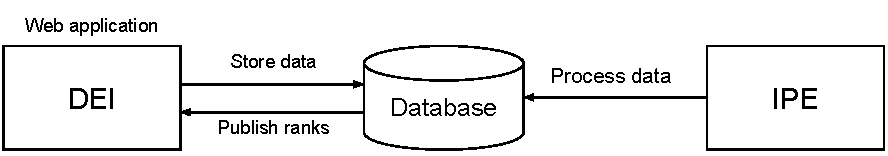
\includegraphics[width=\textwidth]{sloop/system}
  \caption{Score Distribution}
  \label{fig:sloop_overview} %chktex 24
\end{figure}

Sloop is a distributed image retrieval system which comprises three major
components~\cite{sloop14,sloop15,sloopdocs}: \begin{description} \item[Database]
Stores all system data and provides a communication mechanism for the other
parts of the system. There is only one species per deployment.  \item[Data
Exchange and Interaction (DEI)] A web application that provides the user
interface that allows biologists to upload data into Sloop databases.
\item[Image Processing Engine (IPE)] Processes the data stored in the database
and generates descriptors that represent identities of the images.
\end{description} Since we are interested in developing methods for individual
identification, we will be focusing primarily on the IPE.

\subsection{Image Processing Engine (IPE)}

Each species of animal requires different processing techniques.  In skinks
dataset, given an image and the four fiducial key points annotated by the
biologists, Sloop segments the image into thee image patches using the fiducial
keys, and transforms the images into a SIFT object. It then compares the
processed SIFT object with the SIFT objects from the other images stored in the
database. After the ranking is generated, the biologists then look at the top
retrievals and confirm whether the given pairs of images are matches or
non-matches~\cite{sloop14,sloop15}.

One of our goals in this research is to fully automate the feature extraction
process by experimenting with other alternative feature learners because user
assistance in feature extraction is generally considered unnecessary and
expensive. Since all the keypoints in the matching step are weighted equally,
Sloop needs human assistance to locate the discriminating features and exclude
the noises and background. Unlike convolutional neural networks, the weights are
learned directly from the data; thus, very minimal preprocessing is required.

The current version of IPE uses deformation invariant image
matching~\cite{yang09} and SIFT~\cite{lowe04} to perform image matching. While
SIFT is a viable solution for tasks where speed and simplicity are of major
concern, it relies on a tremendous amount of manual feature learning. Matching
such human engineered features, as in SIFT, may lead to poor
generalization~\cite{fisher14}.

% section sloop (end)

\section{Relevance feedback} % (fold)
\label{sec:relevance_feedback}

Relevance Feedback is a technique that involves users in the retrieval process.
Sloop, as an interactive human–machine system, takes advantage of crowd-based
relevance feedback to improve the retrieval results~\cite{sloop15}.
Specifically, given a query that returns a set of initial results, the system
takes user feedback on the initial results to improve the results returned from
the later iterations when given the same or related
queries~\cite{manning2008introduction}.

Not only can user input resolve the errors, it can also be used to train a
machine learning model. The model can incrementally learn from the accumulation
of user-input data in our retrieval system. This creates a positive feedback
loop where the model learns its mistakes from the previous iterations and
re-evaluates its strategy based on the gold standard responses from a human
given at the previous iteration. However, currently, we only focus on the
problem of how we can maximize the information gain from a given amount of user
input.

\subsection{Crowdsourcing}

The crowdsourcing market takes advantage of the collective intelligence of the
online community. In a crowdsourcing market, there are three parties involved:
(1) workers (2) requesters (3) crowdsourcing platform.  \emph{Requesters} submit
tasks with the reward that they are willing to pay \emph{workers} upon the
completion of each task. Some workers may be better than others at certain
tasks. The \emph{platform} provides the environment in which the worker and
requesters interact. All parties gain more information about one another and the
tasks, and make repeated decisions over time.

One problem of our interest is assigning tasks to workers with the goal of
maximizing the quality of completed tasks at a low prices or subject to budget
constraints. As a requester, our utility is the ratio between the amount of
information gain from completed work and the price that we have to pay for the
work. Hence, our problem is to design a mechanism which makes repeated decisions
to maximize our utility.

% section relevance_feedback (end)

% chapter related_work (end)
